\documentclass[10pt]{article}
\usepackage[usenames]{color} %used for font color
\usepackage{amssymb} %maths
\usepackage{amsmath} %maths
\usepackage[utf8]{inputenc} %useful to type directly diacritic characters
\usepackage[letterpaper, portrait, margin=1in]{geometry}
\usepackage{graphicx,wrapfig}
\begin{document}
\subsection*{MSDS610 Week 6 Spark Assignment - Nathan Worsham}
I installed the latest Spark and chose to download the package that was prebuilt for Hadoop 2.6 and later. Then as usual, unpacked it, and created a sym link.
\begin{figure}[!h]
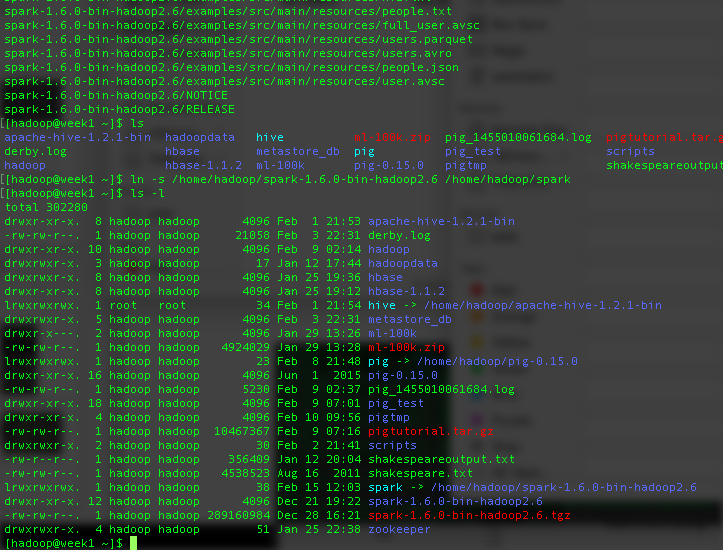
\includegraphics[scale=0.37]{install.png}
\centering
\end{figure}\\
\indent As far as configuration went, it seemed just a couple of environmental variables needed to be set. HADOOP\_CONF\_DIR was already set from last week, so I just set SPARK\_DIST\_CLASSPATH--to \$HADOOP
\_HOME--and SPARK\_LOCAL\_IP to 10.0.2.15. By the end of the assignment I realized I needed/wanted one last environmental variable because I was once again getting a similar warning to week 1--
\begin{verbatim}
Unable to load native-hadoop library for your platform... using builtin-java classes 
where applicable
\end{verbatim}
in week 1 I ended up setting the JAVA\_LIBRARY\_PATH, which was still set but not fixing the problem. I ended up setthing the following to fix it:
\begin{verbatim}
export LD_LIBRARY_PATH=$HADOOP_HOME/lib/native:$LD_LIBRARY_PATH
\end{verbatim}
\indent I then ran the example Scala command it gave of \verb|./bin/run-example SparkPi 10|. Even after scanning the output I wasn't sure what I was supposed to look for or what the script even did. After looking through the actual script, I realized that somewhere in the mash of text that it was supposed to output "Pi is roughly..." and that really is all the example script does is calculate Pi, though I ran the script several times and each time the output is slightly different. I seems that number at the end of the command tells Spark how many processes or threads to split the job into. 
\begin{figure}[!h]
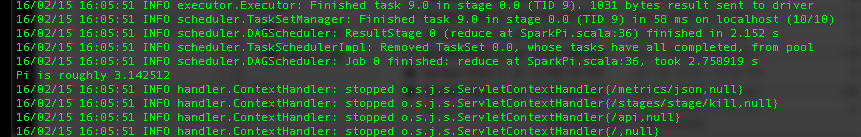
\includegraphics[scale=0.37]{sparkpi.png}
\centering
\end{figure}\\
\indent I went ahead an looked through the scala examples directory but wasn't really sure how to use all of these examples. I did go ahead and try running the SplarkALS example in the same manner as the SparkPi example. This did seem to work, it outputted an RMSE (root-mean-square-error) value from 5 iterations. Though I'm not sure what the values indicate.
\par
\raisebox{-.6\height}{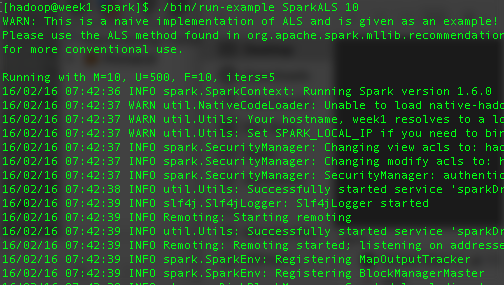
\includegraphics[width=8cm]{ALS1.png}}%
\hfill
\raisebox{-.6\height}{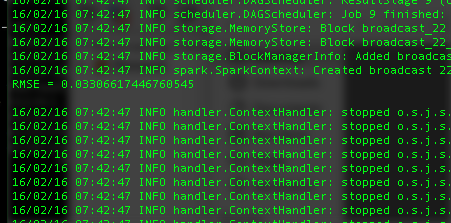
\includegraphics[width=8cm]{ALS2.png}}%
\par
\indent As another test I tried running the Python IDLE in spark, which worked as expected.
\begin{figure}[!h]
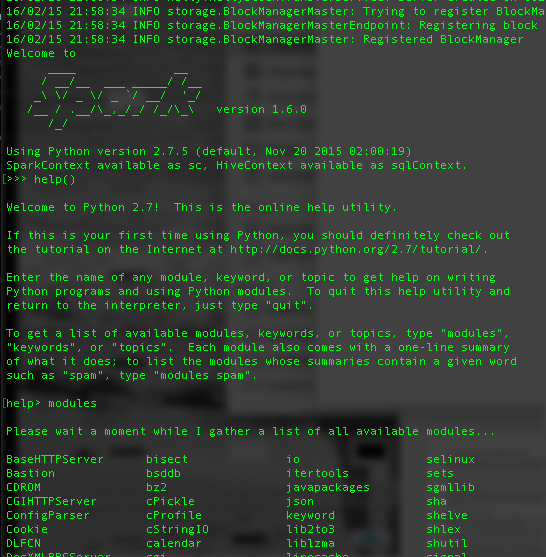
\includegraphics[scale=0.37]{pyspark.png}
\centering
\end{figure}\\
\subsection*{Scala Shell}
I connected to the Scala shell as directed and it worked as expected. I am not familiar with scala, but looking it up on the internet seems it is a programming language whose name means "scalable language" (scala-lang.org, 2016). Continuing on, it appears that \verb|val| must set a variable or object and I successfully set the readme file to the \verb|textFile| object. However when I tried the next line to count the words in the file I received and error about the input path not existing in the HDFS.
\begin{figure}[!h]
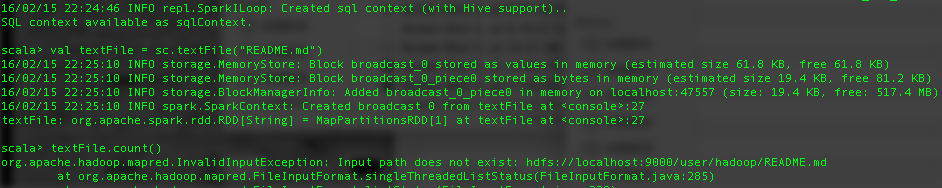
\includegraphics[scale=0.37]{input_path.png}
\centering
\end{figure}\\
\indent I went ahead and using \verb|copyFromLocal|, copied the file to the HDFS but again received the same error. I came across a stackoverflow.com (2014) thread that had a very similar problem, the solution was to use \verb|"file:///home/hadoop/spark/README.md"| instead of just \verb|"README.md"|. I went ahead and tried this but the first time I did not put enough forward slashes and received an error message of 
\begin{verbatim}
Wrong FS: file://home/hadoop/spark/README.md, expected: file:///
\end{verbatim}
After I did it correctly, this time I received the correct output. Although the number for "Long" I received was 95 and not 126 like the example stated. I decided one way to confirm this was correct was to run the python version it provides and sure enough I received 95 as well.
\par
\raisebox{-.6\height}{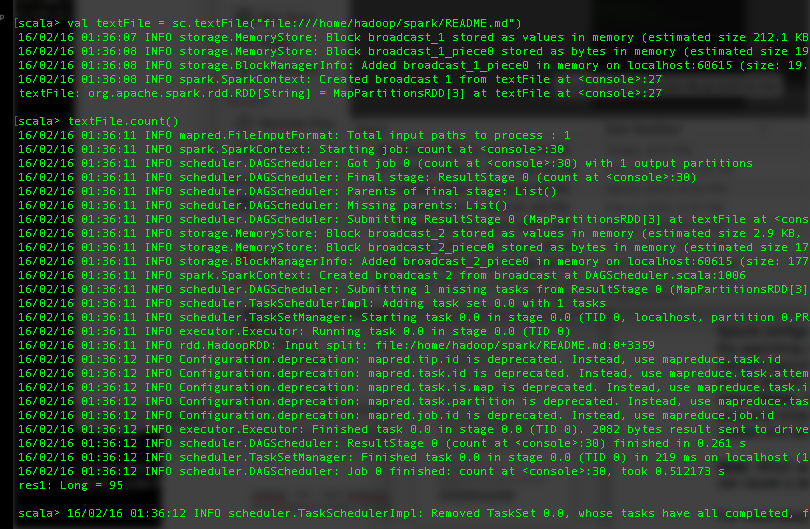
\includegraphics[width=8cm]{full_path.png}}%
\hfill
\raisebox{-.6\height}{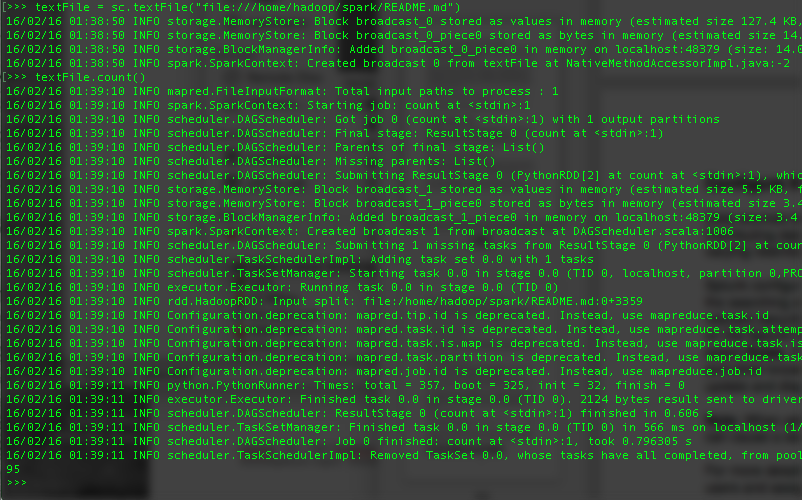
\includegraphics[width=8cm]{fullp_python.png}}%
\par
Next I confirmed that "Apache Spark" is the first item.
\begin{figure}[!h]
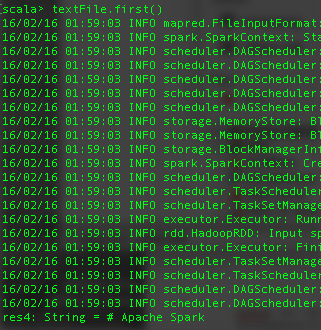
\includegraphics[scale=0.37]{first.png}
\centering
\end{figure}\\
\indent The remaining portion of the "Basics" section did not make a lot of sense to me. First it asks you to create a variable or value with the text file filtered with lines that contain "Spark"--which worked fine. But in the following command it ignores the variable just created and uses the filter again then \verb|.count()| on the end. I went ahead and did it their way first, which returned 17 as an answer, but then I tried it as \verb|linesWithSpark.count()| which returned the same value. 
\begin{figure}[!h]
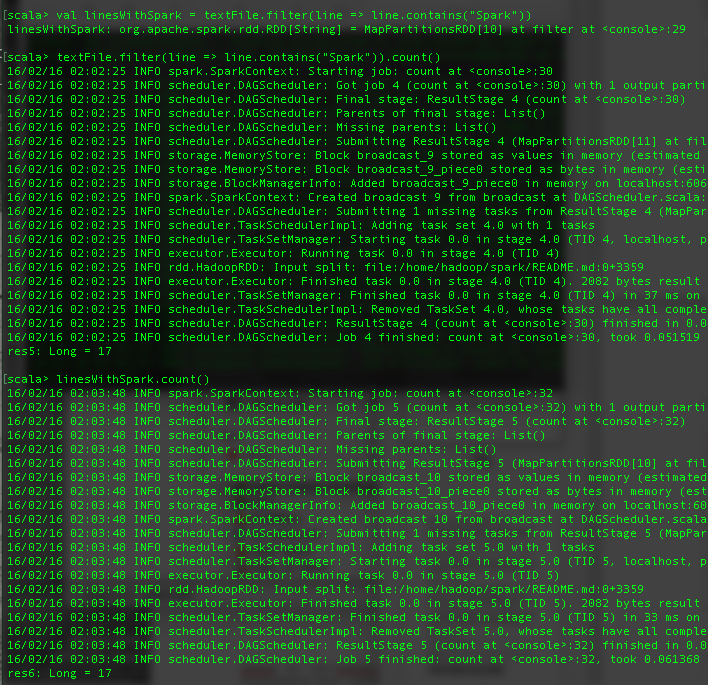
\includegraphics[scale=0.33]{linesWithSpark.png}
\centering
\end{figure}\\
\indent For the "More on RDD Operations" section, I received the answer of line 14 being the longest, however I found it fairly tough trying to understand the command they gave. I even took a look at the Python version--since I am more familiar with Python--but that seemed even more cryptic. The exercise goes on to say to make the command "easier" to understand it uses the \verb|Math.max()|function but again I'm not familiar with it, so it doesn't clear up much for me but does confirm the same output of 14. That being said, looking at the Python version of the example, it shows it using a custom function instead and the function is much easier to read.
\par
\raisebox{-.6\height}{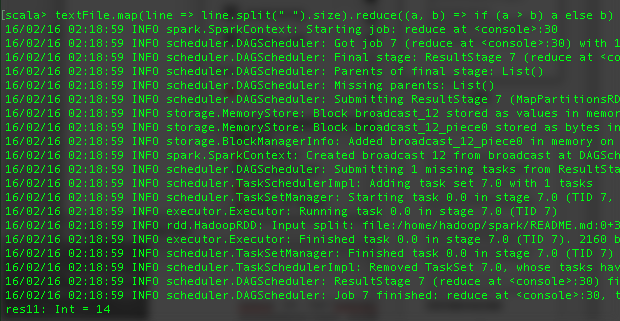
\includegraphics[width=8cm]{reduce.png}}%
\hfill
\raisebox{-.6\height}{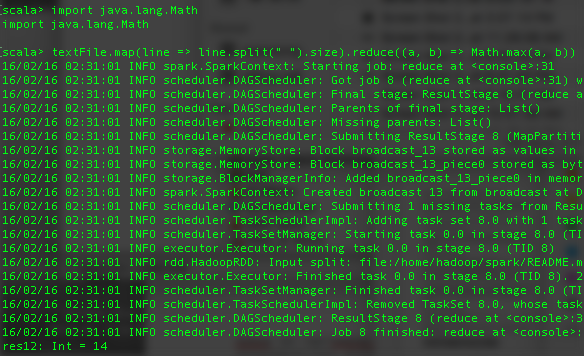
\includegraphics[width=8cm]{mathmax.png}}%
\par
Finally I did the per-word counts as directed. I found it strange that the output was cut off. 
\begin{figure}[!h]
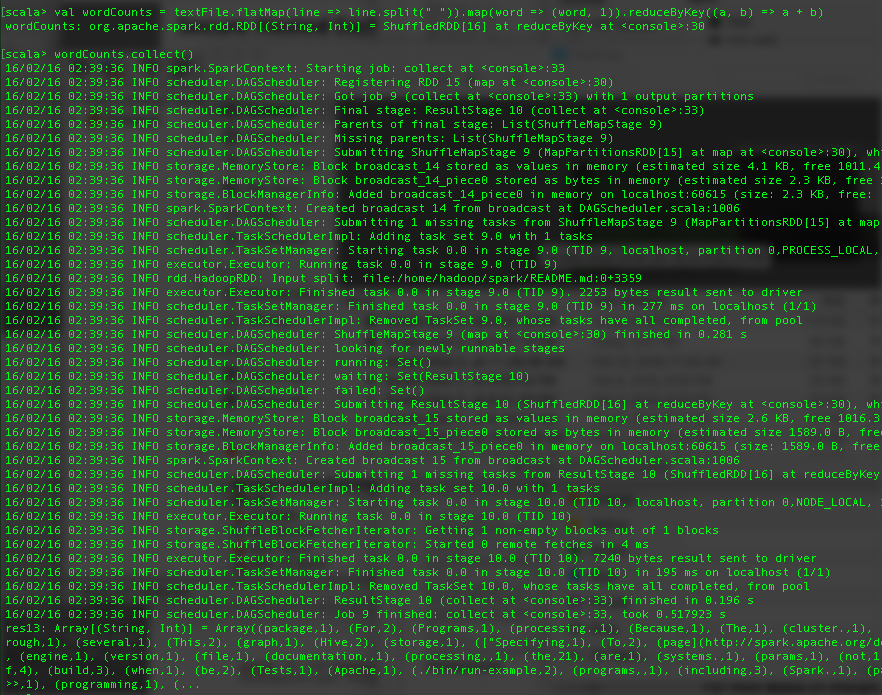
\includegraphics[scale=0.37]{wordCounts.png}
\centering
\end{figure}\\
\indent I found I could list all of the output using \verb|println(wordCountsResults.deep.mkString("\n"))|.
\pagebreak
\begin{figure}[!h]
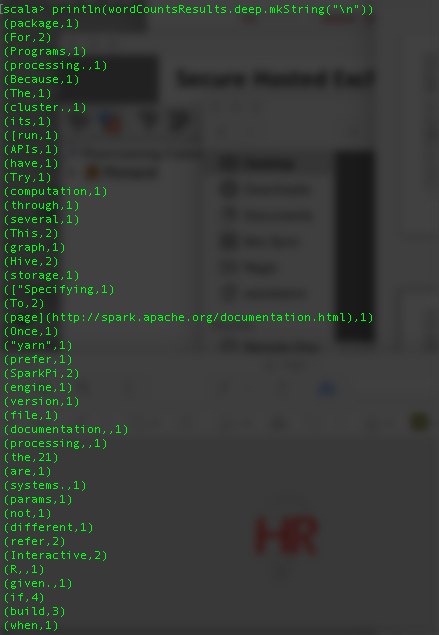
\includegraphics[scale=0.37]{notCutOff.png}
\centering
\end{figure}\\
\subsection*{References}
scala-lang.org, 2016. Retrieved from http://www.scala-lang.org/what-is-scala.html\\
stackoverflow.com, 2014. Retrieved from http://stackoverflow.com/questions/27299923/how-to-load-local-file-in-sc-textfile-instead-of-hdfs\\
stackoverflow.com, 2010. Retrieved from http://stackoverflow.com/questions/3328085/scala-printing-arrays\\
spark.apache.org, n.d. Retrieved from http://spark.apache.org/docs/latest
\end{document}
